\chapter{Screenshots of Issie 3.0.0} \label{app:screenshots}
Screenshots taken on MacOS.

\begin{figure} [h]
    \centering
    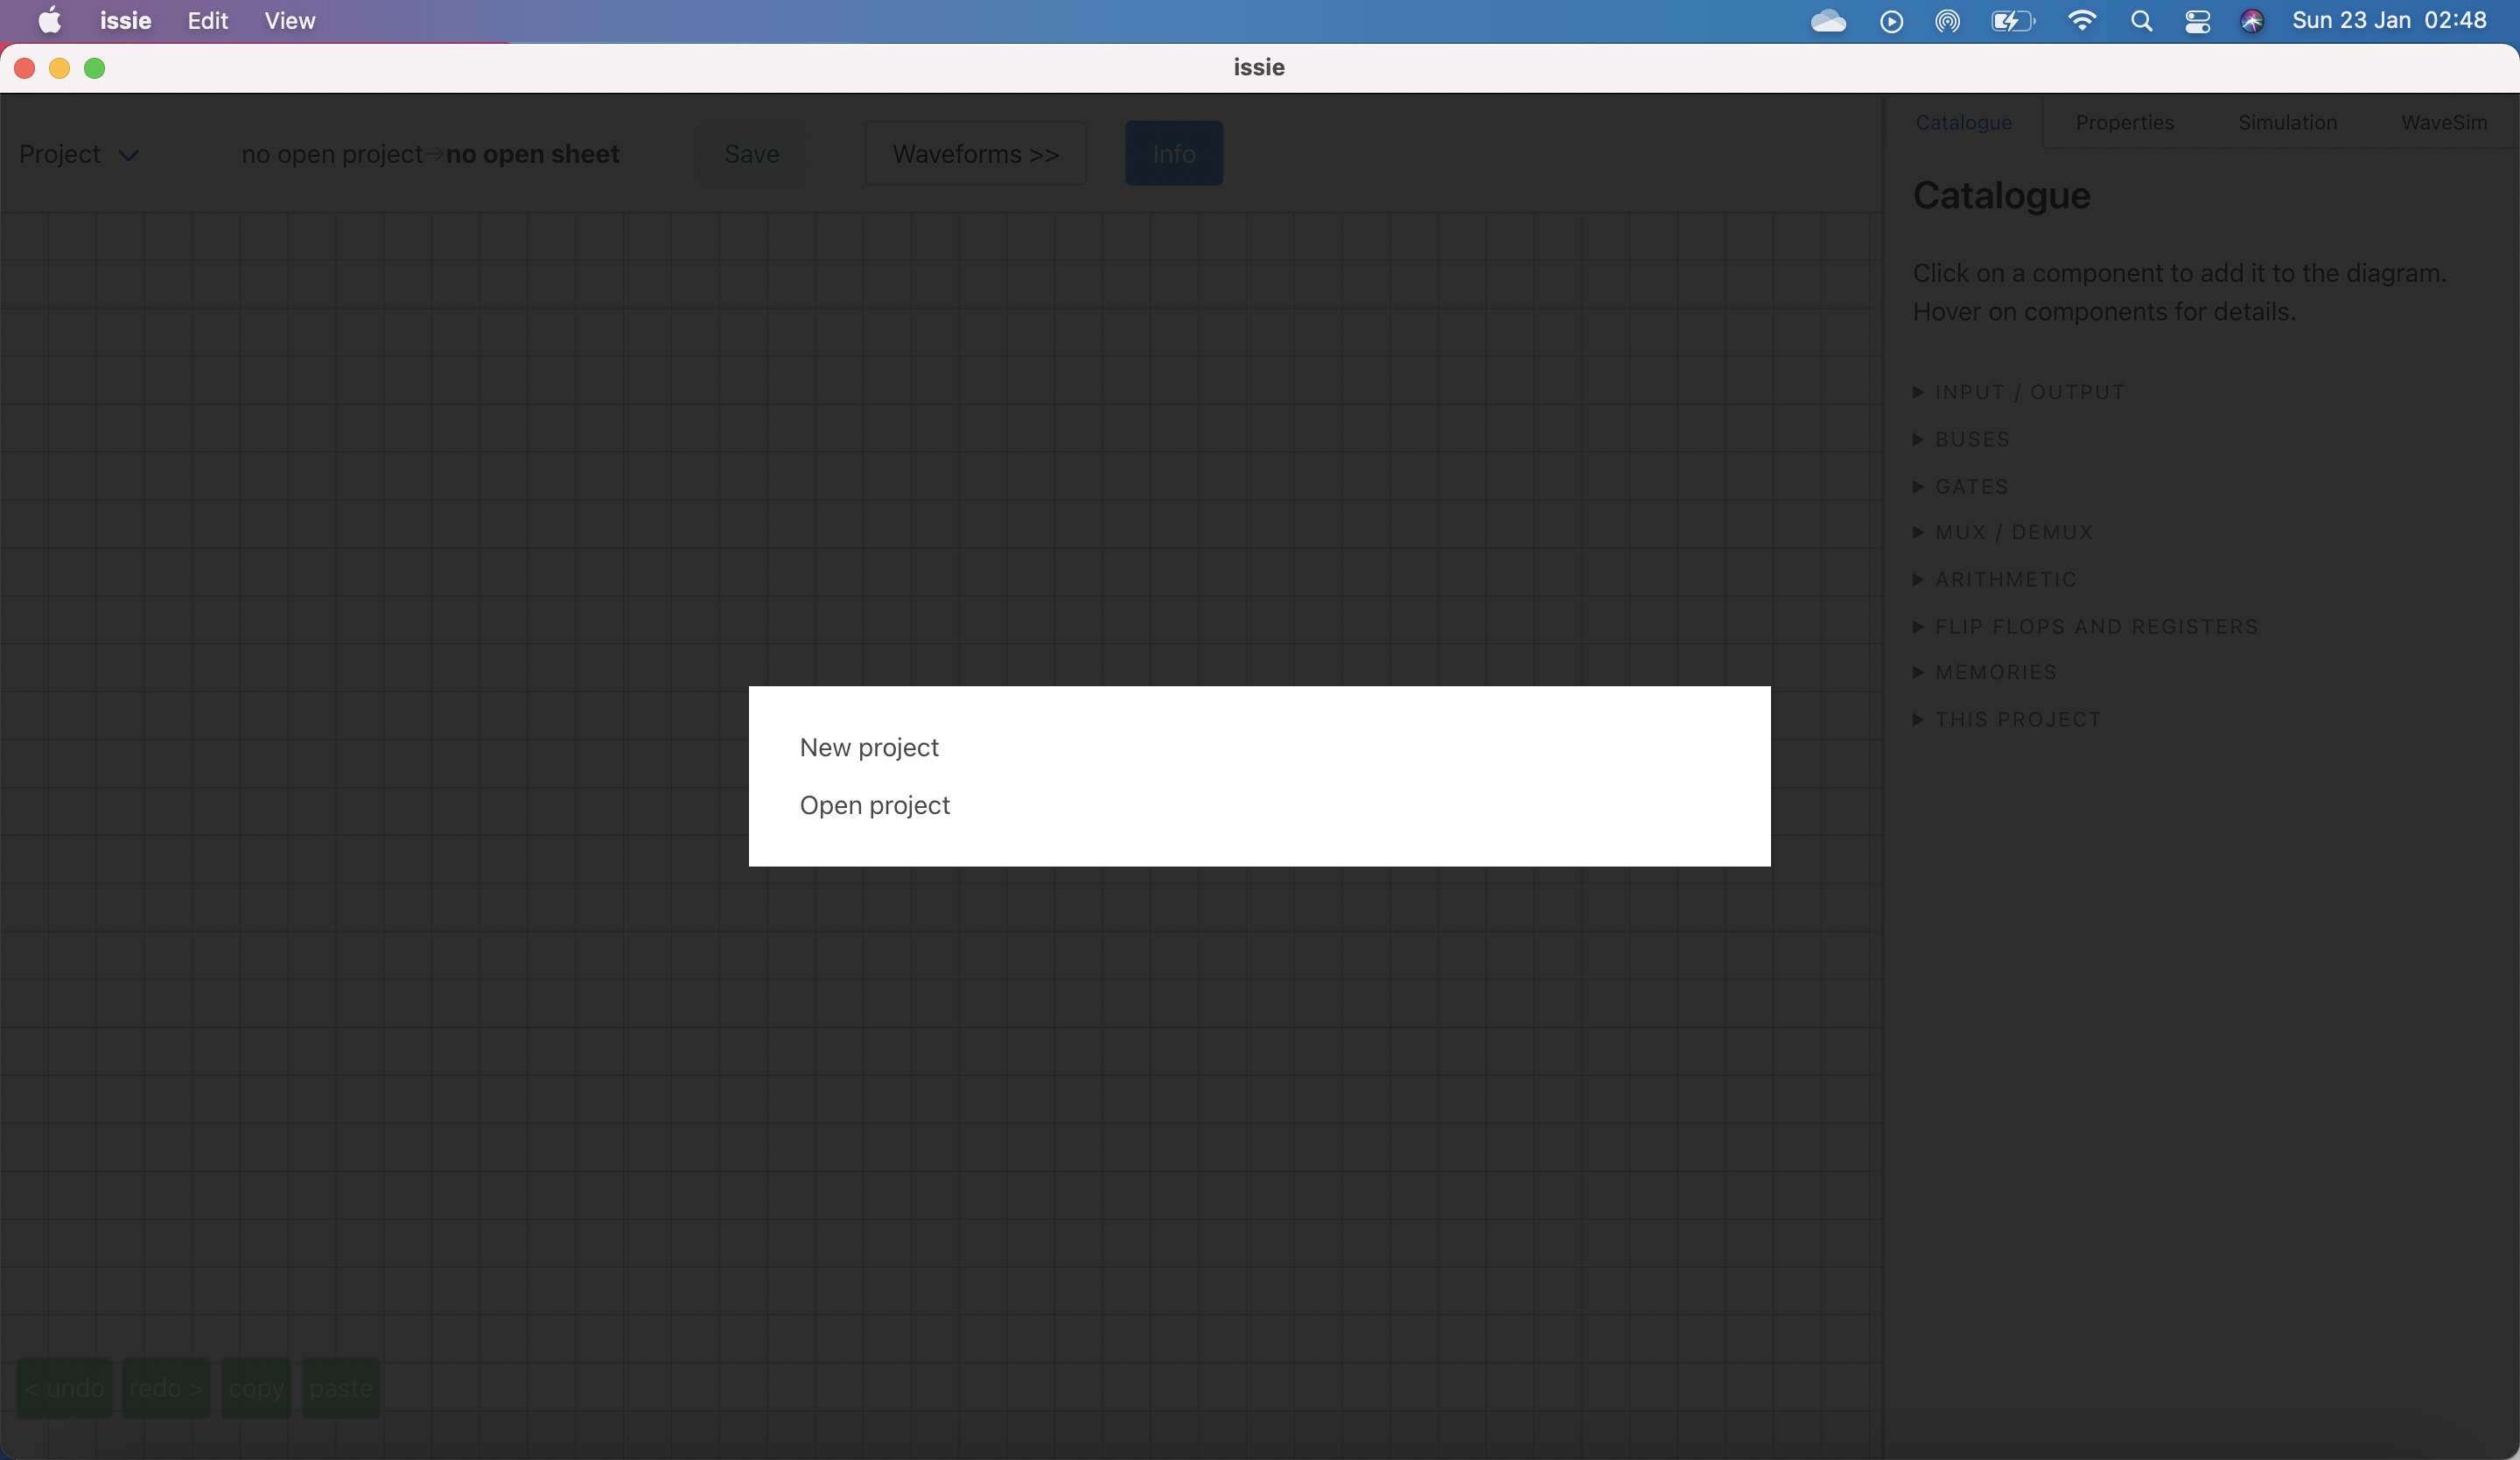
\includegraphics[width=\textwidth]{Appendices/IssieOpening.png}
    \caption{Issie's opening screen}
    \label{fig:IssieOpen}
\end{figure}

\begin{figure} [h]
    \centering
    \includegraphics[width=\textwidth]{Appendices/IssieSheetAnnotated.png}
    \caption{A sheet (schematic) open in Issie, with a component and wire selected}
    \label{fig:IssieSheetAnnotated}
\end{figure}

\begin{figure} [h]
    \centering
    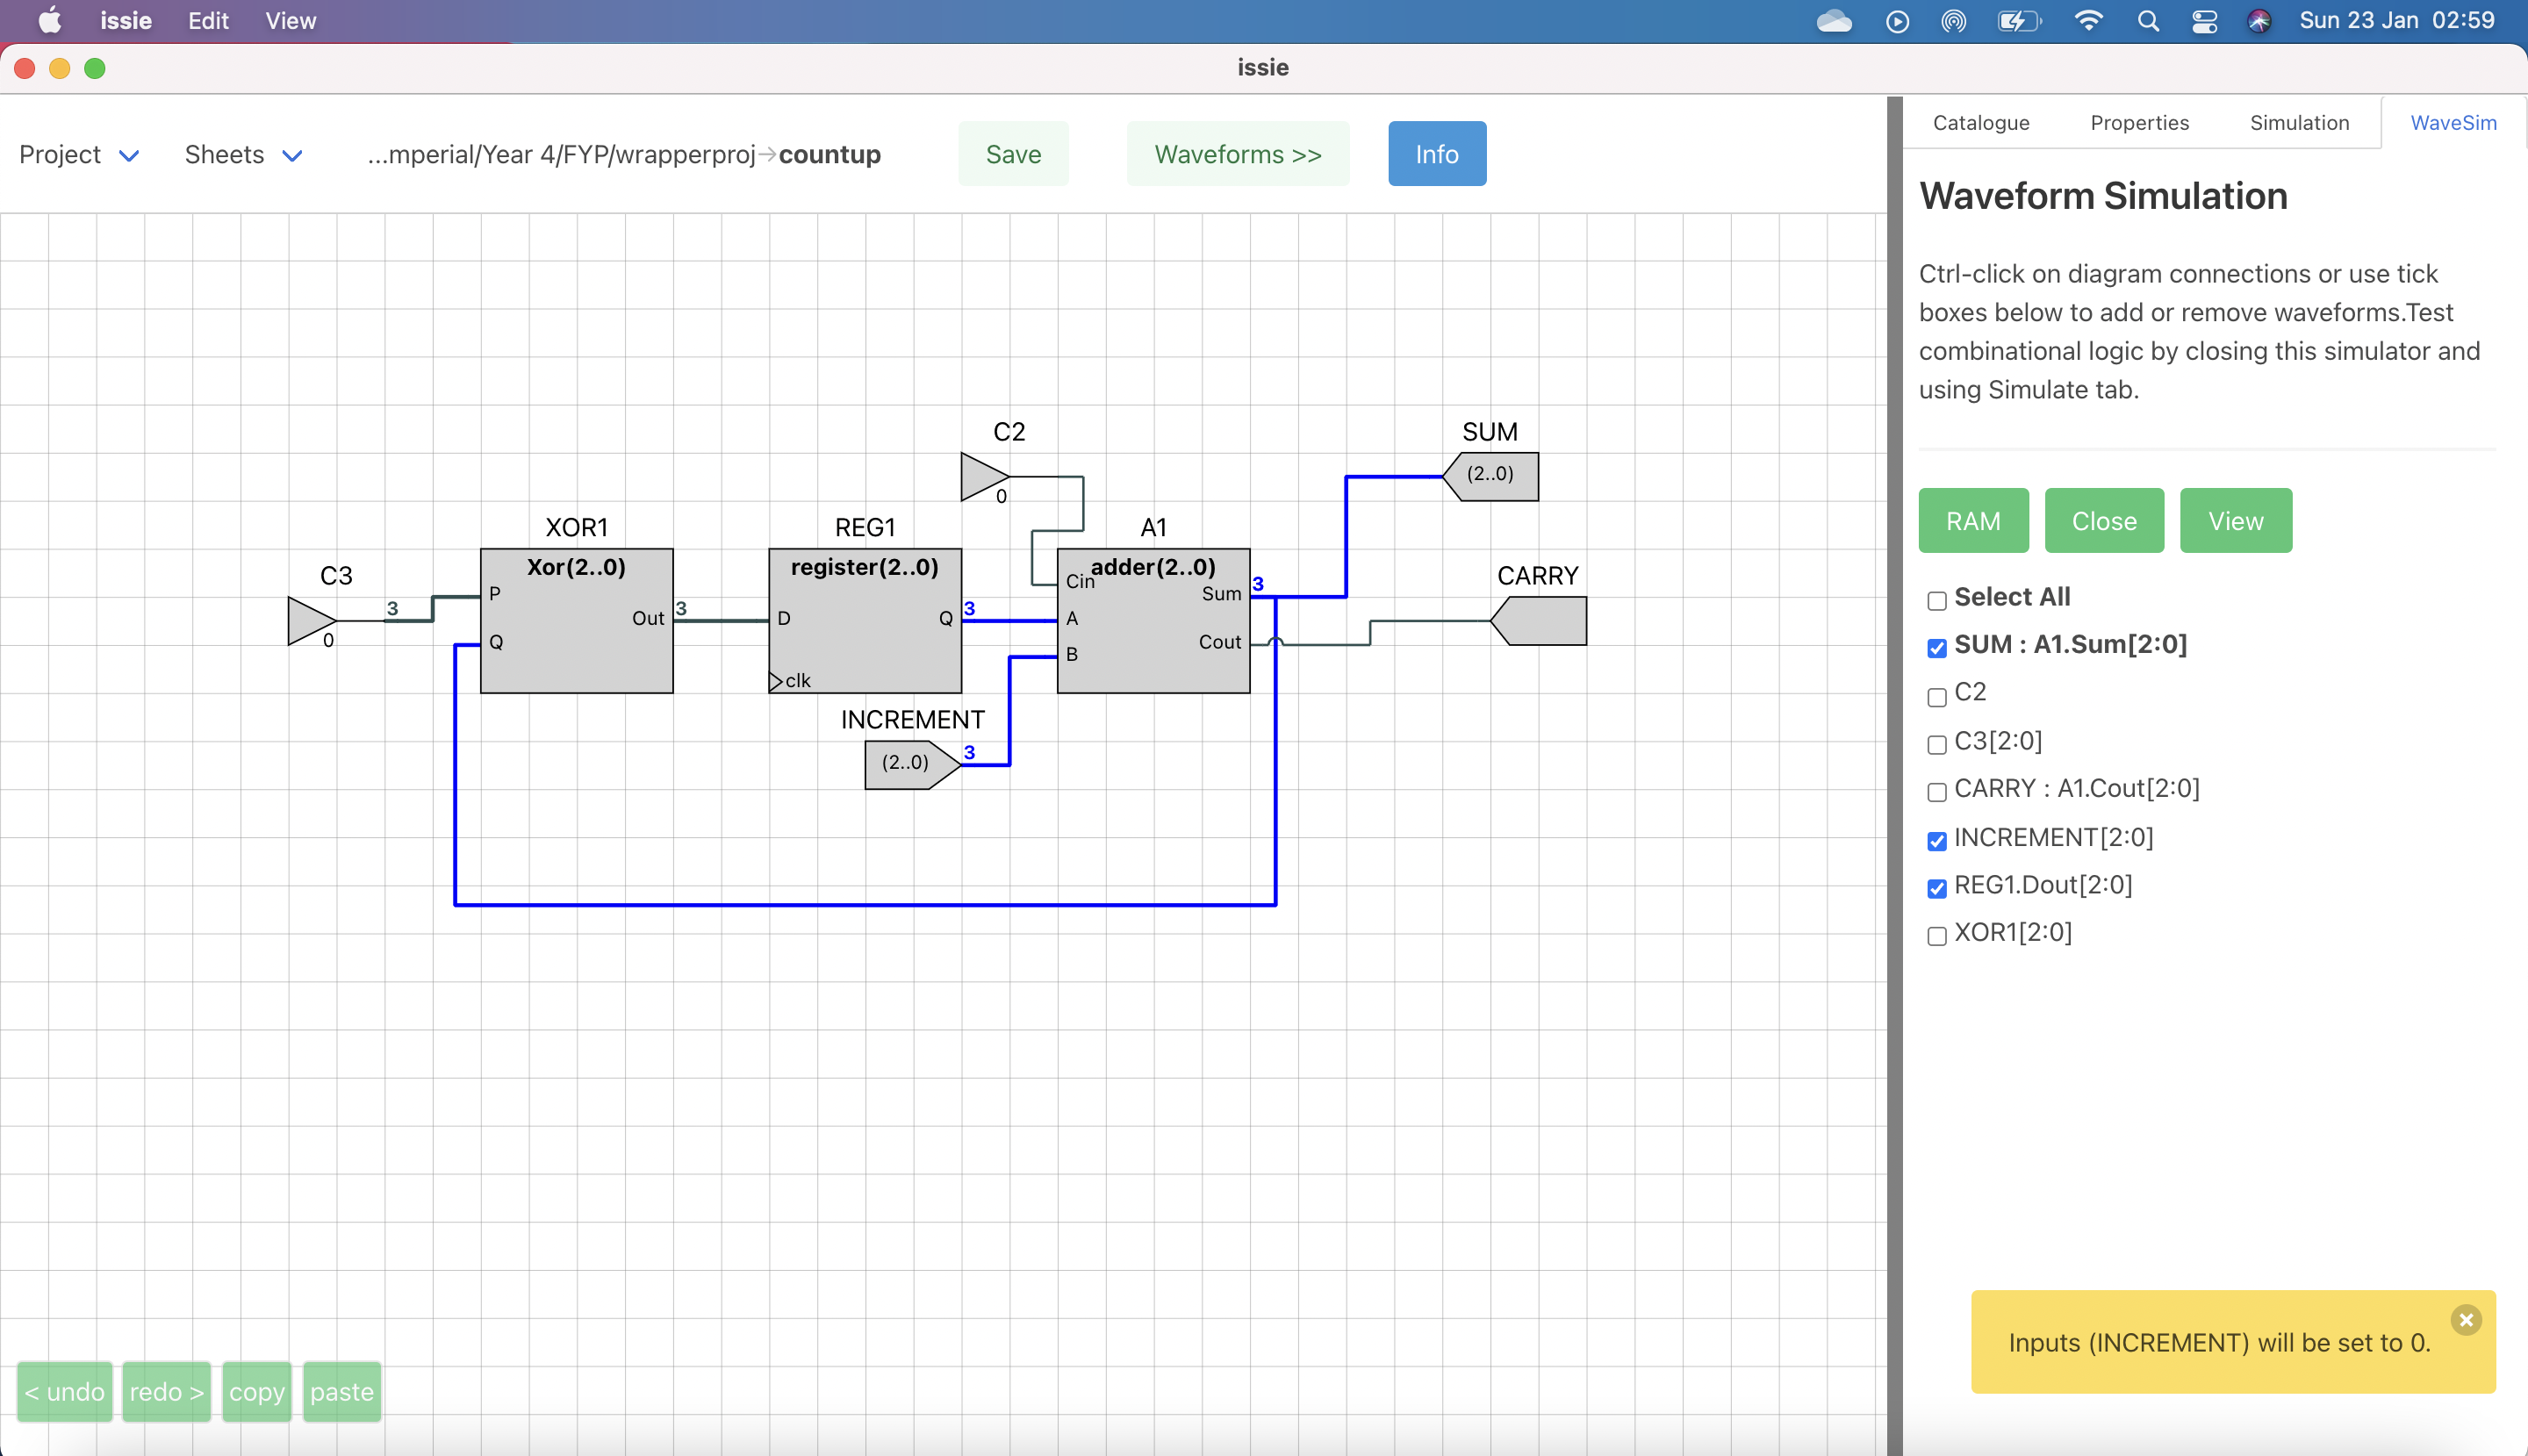
\includegraphics[width=\textwidth]{Appendices/IssieWaveSimSel.png}
    \caption{Issie's Waveform Simulator selection menu}
    \label{fig:IssieWSSel}
\end{figure}

\begin{figure} [h]
    \centering
    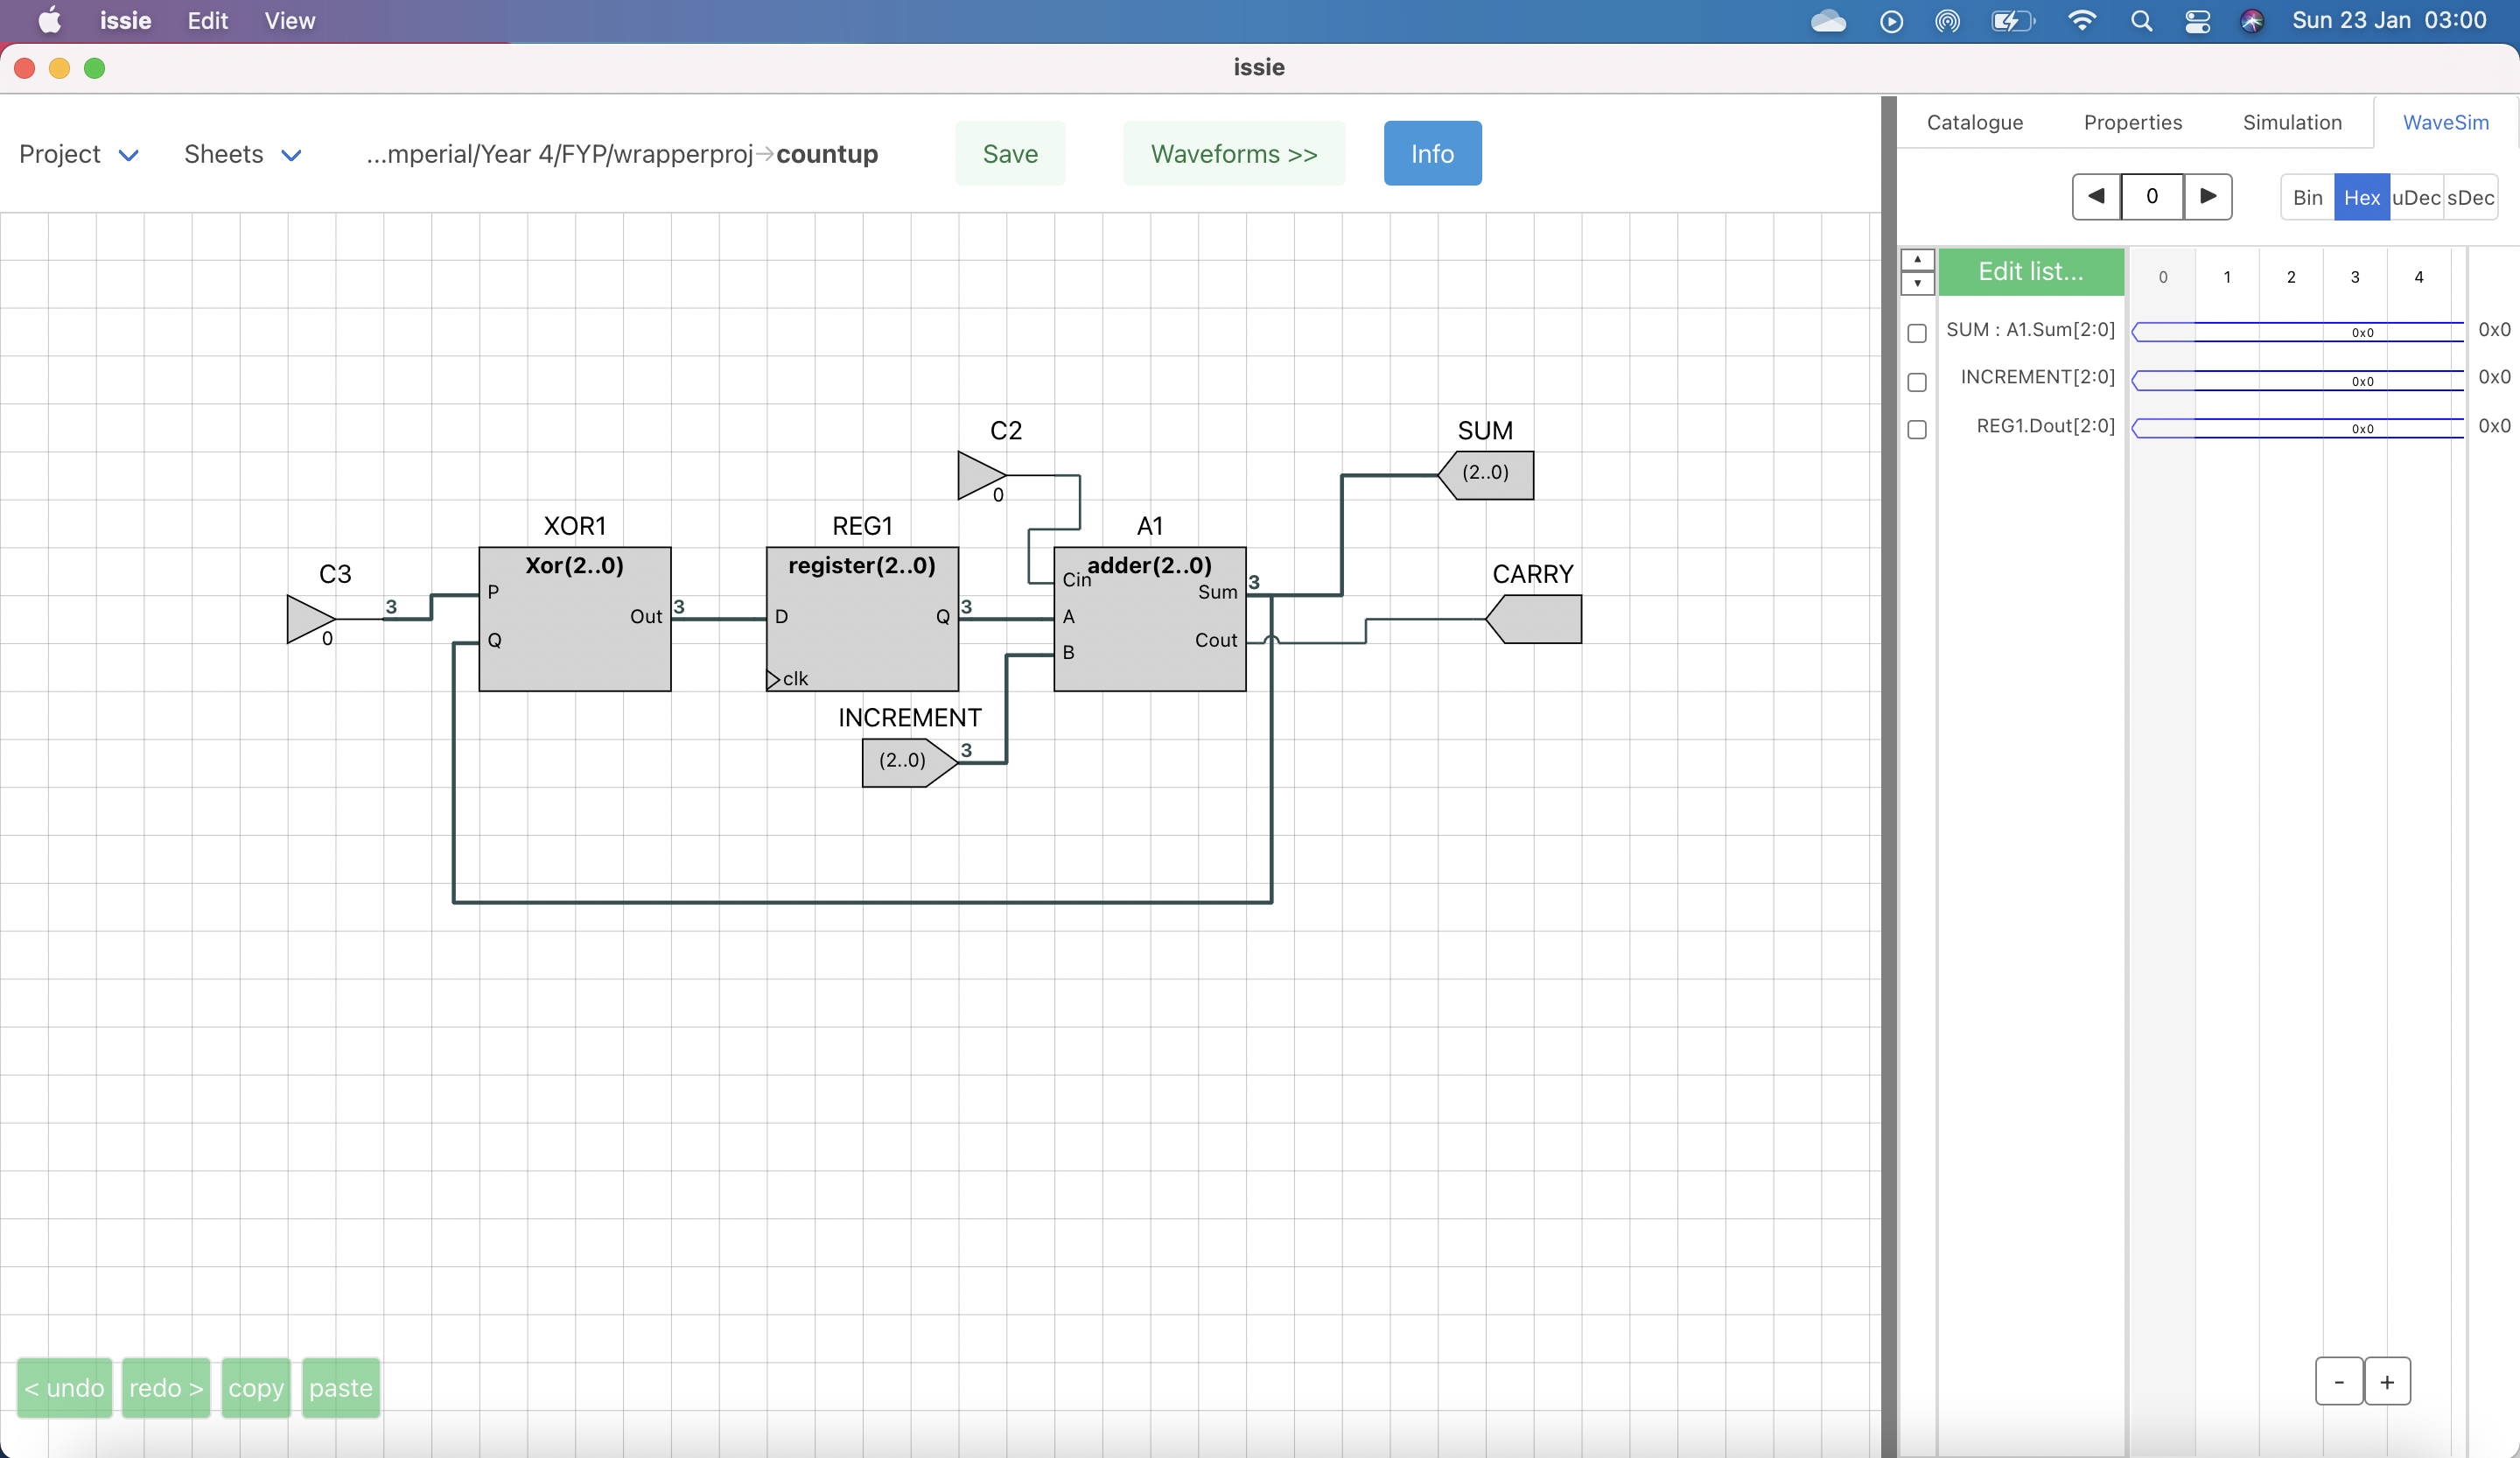
\includegraphics[width=\textwidth]{Appendices/IssieWaveSim.png}
    \caption{Issie's Waveform Simulator}
    \label{fig:IssieWS}
\end{figure}

\chapter{Work Breakdown Structure} \label{app:wbs}
\begin{figure}
    \centering
    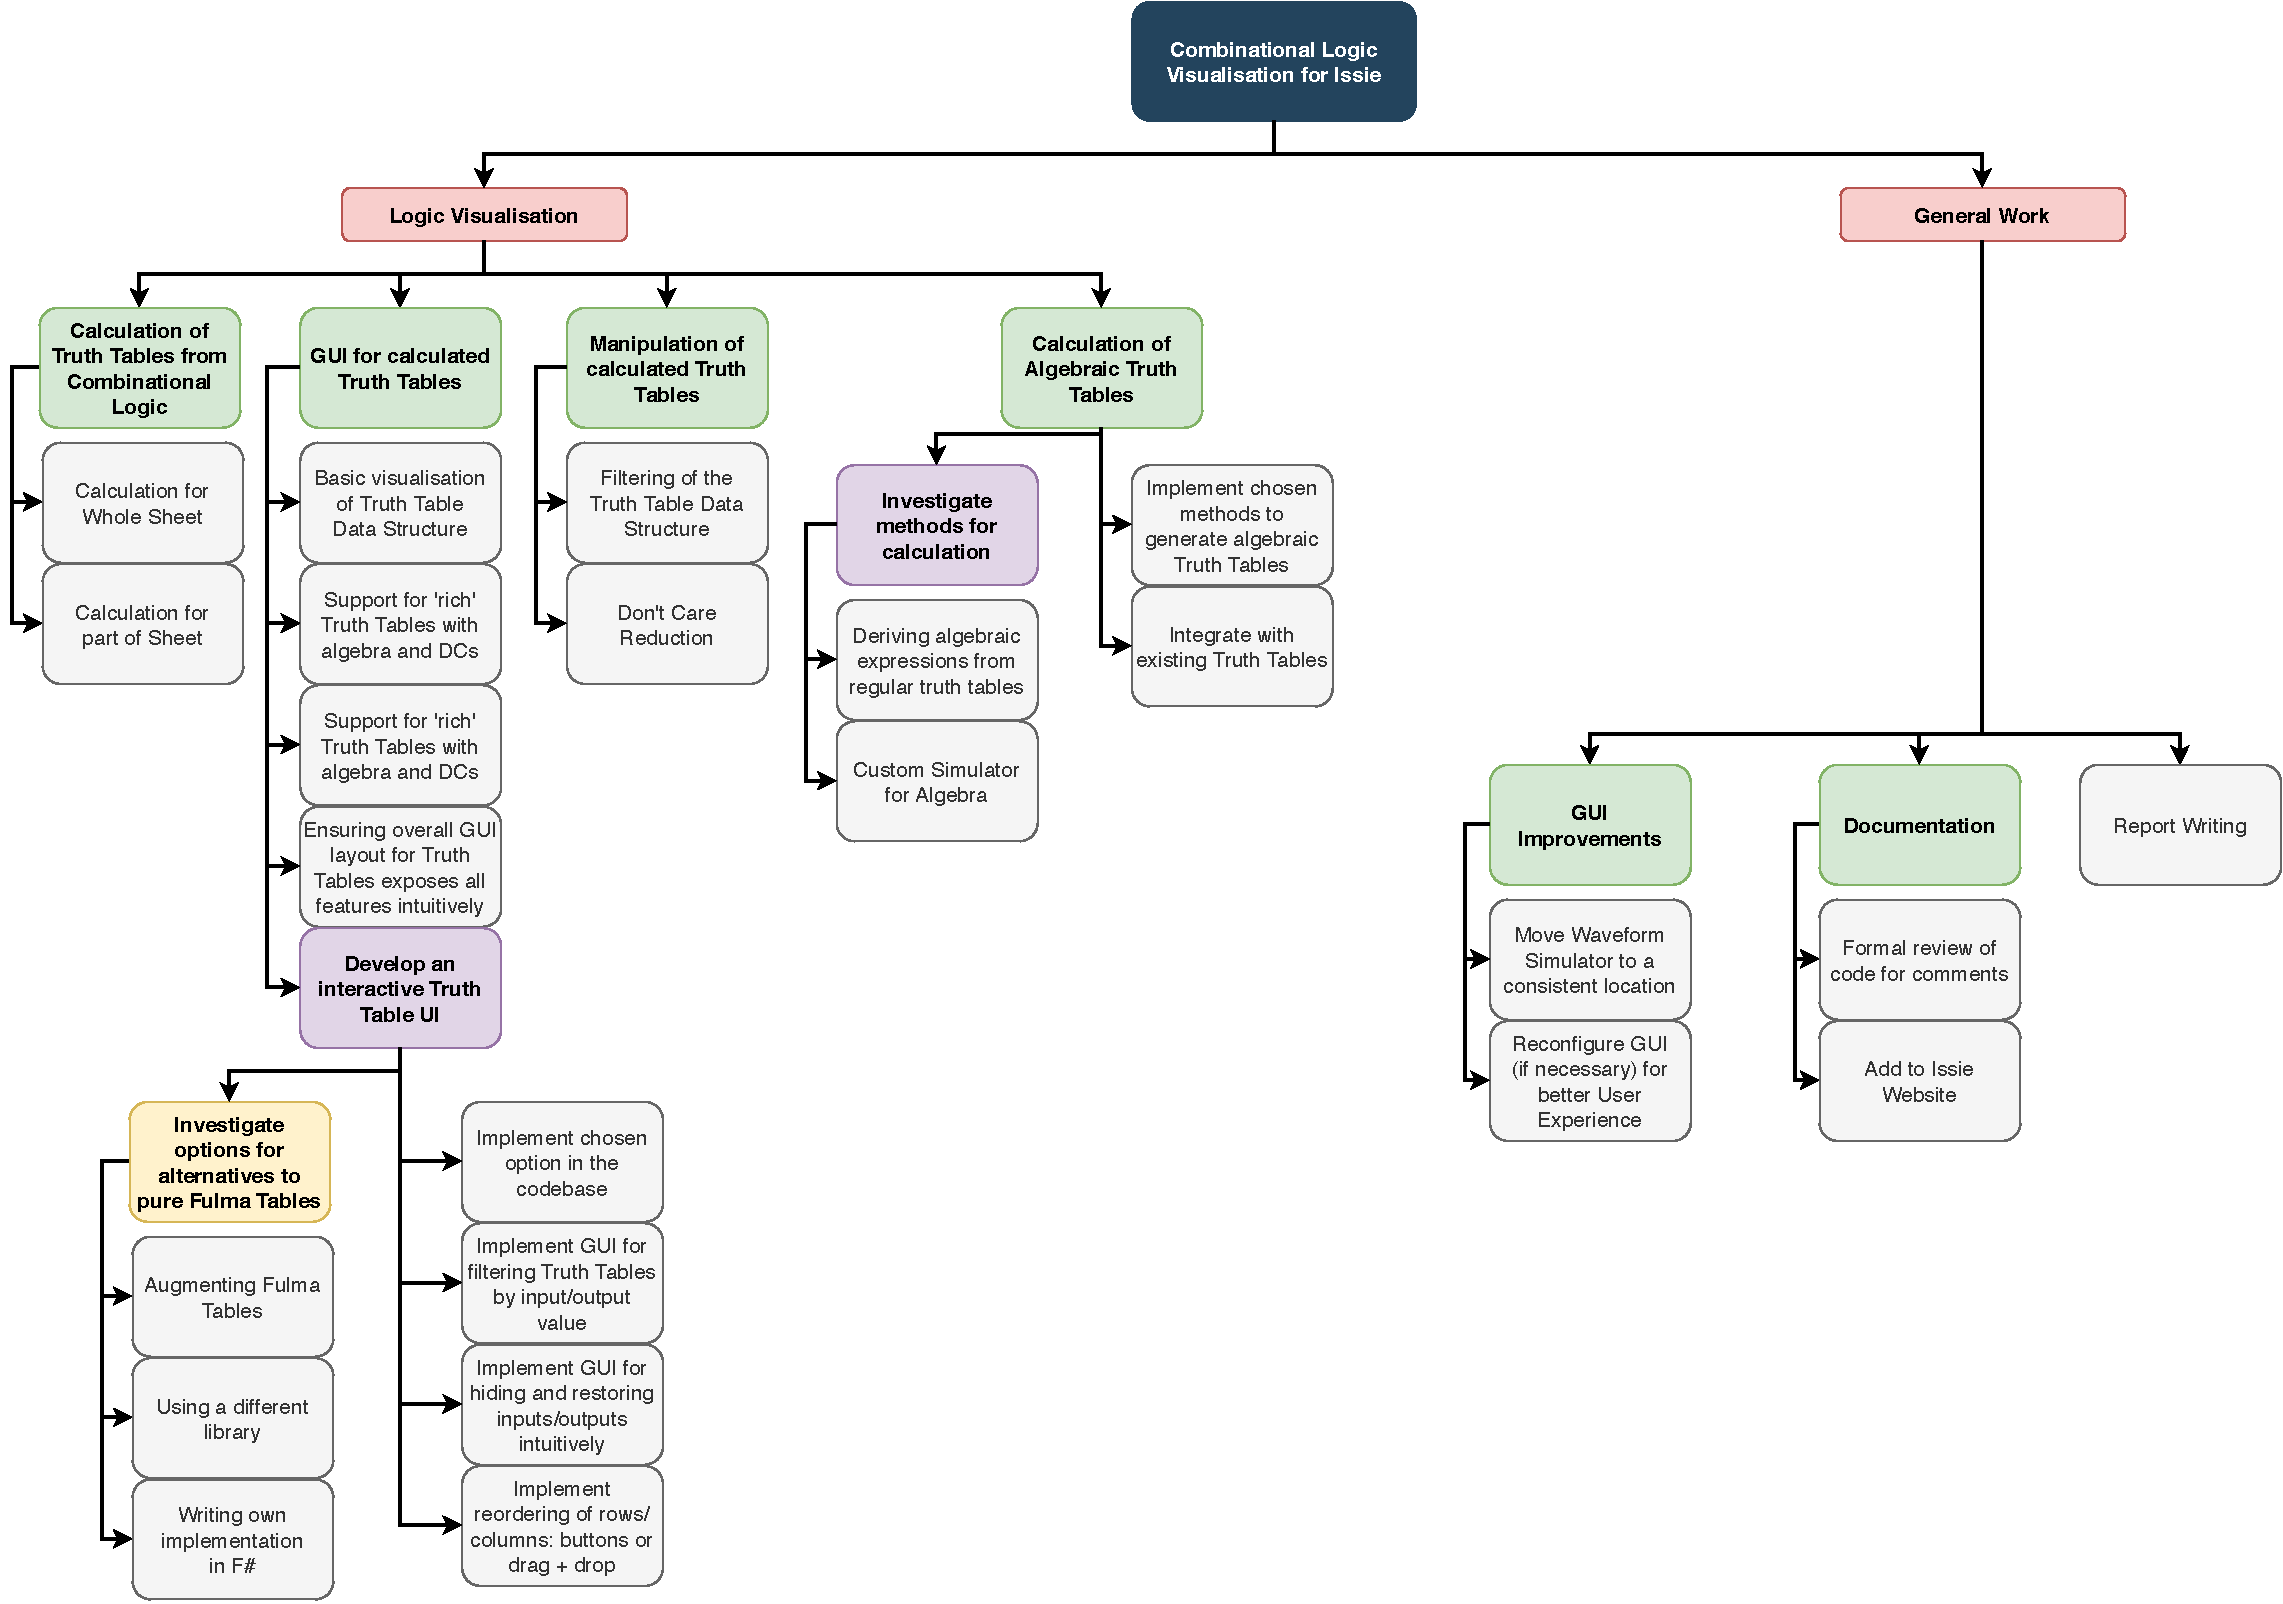
\includegraphics{Appendices/wbs2.pdf}
    \caption{Work Breakdown Structure with ordered backlog}
    \label{fig:wbs2}
\end{figure}

\chapter{8-bit ALU Schematic} \label{app:alu}
\begin{figure}
    \centering
    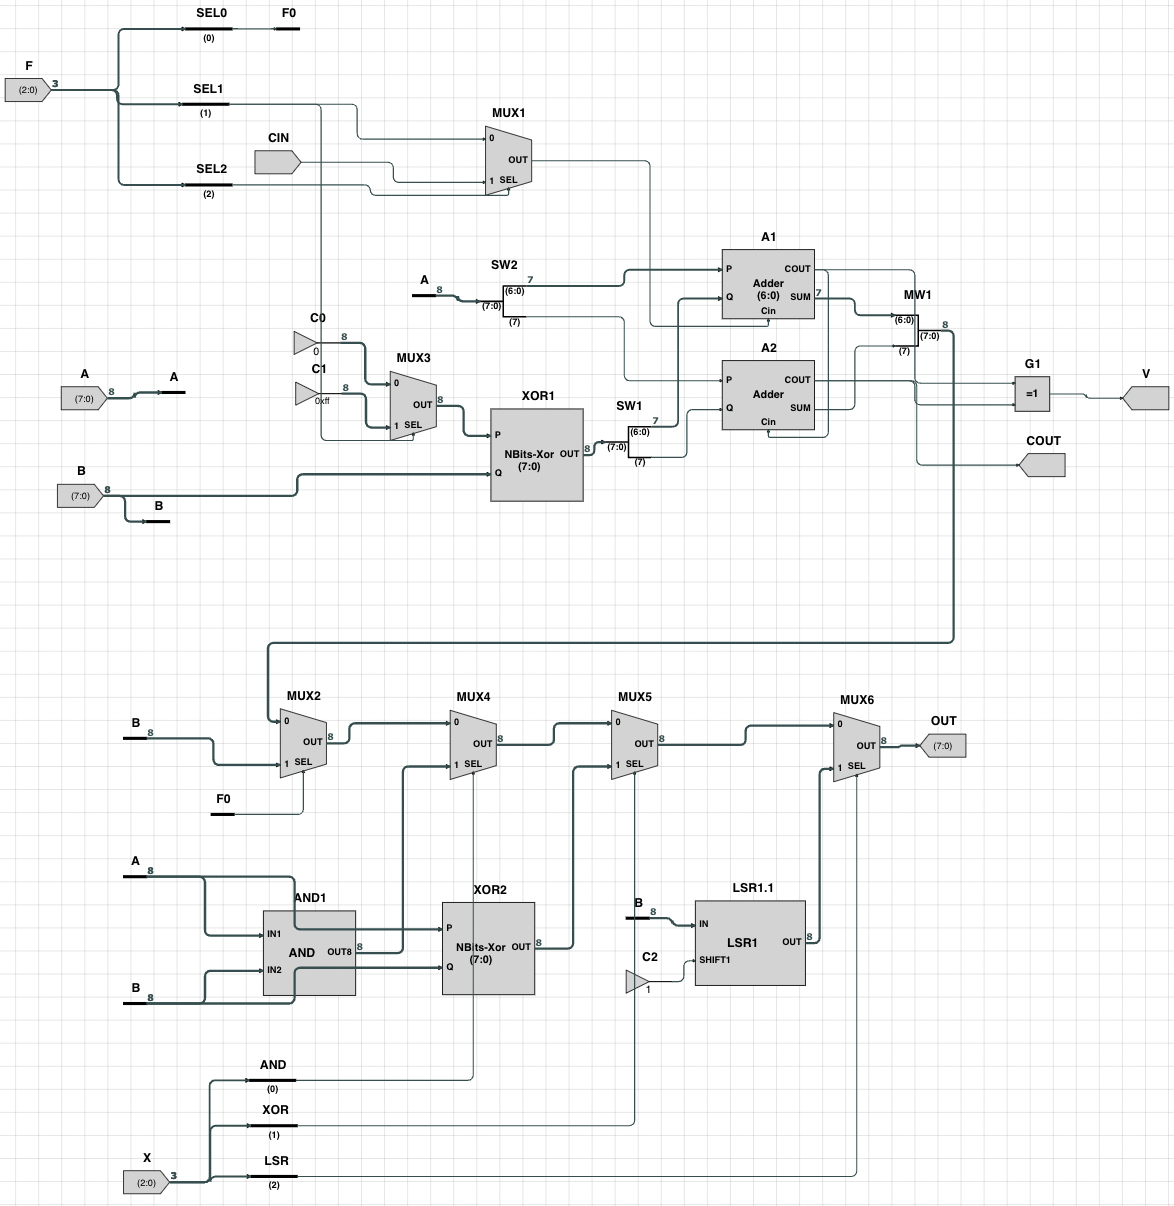
\includegraphics[width=\textwidth]{Appendices/alu8bit.png}
    \caption{Schematic Diagram for an 8-bit ARM ALU}
    \label{fig:alu8bit}
\end{figure}
